\documentclass{beamer}

\usepackage{graphicx}
\usepackage[T1]{fontenc}
\usepackage[english]{babel}
\usepackage{listings}
%\lstloadlanguages{R}
%\lstset{ %
%	language=R,                % the language of the code
%	basicstyle=\footnotesize,           % the size of the fonts that are used for the code
%	numbers=left,                   % where to put the line-numbers
%	numberstyle=\tiny\color{gray},  % the style that is used for the line-numbers
%	stepnumber=2,                   % the step between two line-numbers. If it's 1, each line
%	% will be numbered
%	numbersep=5pt,                  % how far the line-numbers are from the code
%	backgroundcolor=\color{yellow},      % choose the background color. You must add \usepackage{color}
%	showspaces=false,               % show spaces adding particular underscores
%	showstringspaces=false,         % underline spaces within strings
%	showtabs=false,                 % show tabs within strings adding particular underscores
%	frame=single,                   % adds a frame around the code
%	rulecolor=\color{black},        % if not set, the frame-color may be changed on line-breaks within not-black text (e.g. commens (green here))
%	tabsize=2,                      % sets default tabsize to 2 spaces
%	captionpos=b,                   % sets the caption-position to bottom
%	breaklines=true,                % sets automatic line breaking
%	breakatwhitespace=false,        % sets if automatic breaks should only happen at whitespace
%	title=\lstname,                   % show the filename of files included with \lstinputlisting;
%	% also try caption instead of title
%	keywordstyle=\color{blue},          % keyword style
%	commentstyle=\color{dkgreen},       % comment style
%	stringstyle=\color{mauve},         % string literal style
%	escapeinside={\%*}{*)},            % if you want to add a comment within your code
%	morekeywords={*,...}               % if you want to add more keywords to the set
%}
\lstset{commentstyle=\color{red},keywordstyle=\color{black},
	showstringspaces=false}
\lstnewenvironment{rc}[1][]{\lstset{language=R}}{}
\newcommand{\ri}[1]{\lstinline{#1}}  %% Short for 'R inline'

\lstset{language=R}             % Set R to default language

\usepackage{xcolor}
\usepackage{eso-pic}
\usepackage{mathrsfs}
\usepackage{url}
\usepackage{amssymb}
\usepackage{amsmath}
\usepackage{multirow}
\usepackage{hyperref}
\usepackage{booktabs}
\usepackage{bbm}
\usepackage{cooltooltips}
\usepackage{colordef}
\usepackage{beamerdefs}
\usepackage{lvblisting}
\usepackage{textcomp}
\usepackage{inputenc}

\pgfdeclareimage[height=3.5cm]{logobig}{hulogo}
\pgfdeclareimage[height=0.7cm]{logosmall}{Rlogo}

\renewcommand{\titlescale}{1.0}
\renewcommand{\titlescale}{1.0}
\renewcommand{\leftcol}{0.6}

\title[Introduction to R]{Introduction to R}
\authora{Martin Weber}
\authorb{Awdesch Melzer}
\authorc{}

\def\linka{http://wiwi.hu-berlin.de/finanz}
\def\linkb{}
\def\linkc{}

\institute{Institute of Finance\\
	Humboldt-Universit\"at zu Berlin\\}

\hypersetup{pdfpagemode=FullScreen}

\begin{document}

% 0-1
%%%%%%%%%%%%%%%%%%%%%%%%%%%%%%%%%%%%%%%%
\frame[plain]{
\titlepage
}

%%%%%%%%%%%%%%%%%%%%%%%%%%%%%%%%%%%%%%%%
\section{Introduction}
\frame{
\frametitle{What is 
\includegraphics[scale=0.1]{Rlogo}?}
\begin{itemize}
	\item S language, developed by R. Becker and J. Chambers in 1984
  \item GNU implementation of S 1992 by R. Ihaka and R. Gentleman
in NZ
  \item great variety of packages covering all fields of statistics
  \item non-commercial use mostly for free
\end{itemize}
}





%%%%%%%%%%%%%%%%%%%%%%%%%%%%%%%%%%%%%%%%


% 1-2
%%%%%%%%%%%%%%%%%%%%%%%%%%%%%%%%%%%%%%%%
\frame{
\frametitle{What can 
\includegraphics[scale=0.1]{Rlogo} \;\,do?}
\begin{columns}
	\begin{column}{0.4\textwidth}
		\begin{itemize}
			\item {\large Empirical modelling}
			\item {\large Visualisation}
			\item {\large Simulations}
			\item {\large Interactive analysis}
			\item \ldots
		\end{itemize}
	\end{column}
	\begin{column}{0.59\textwidth}
	
	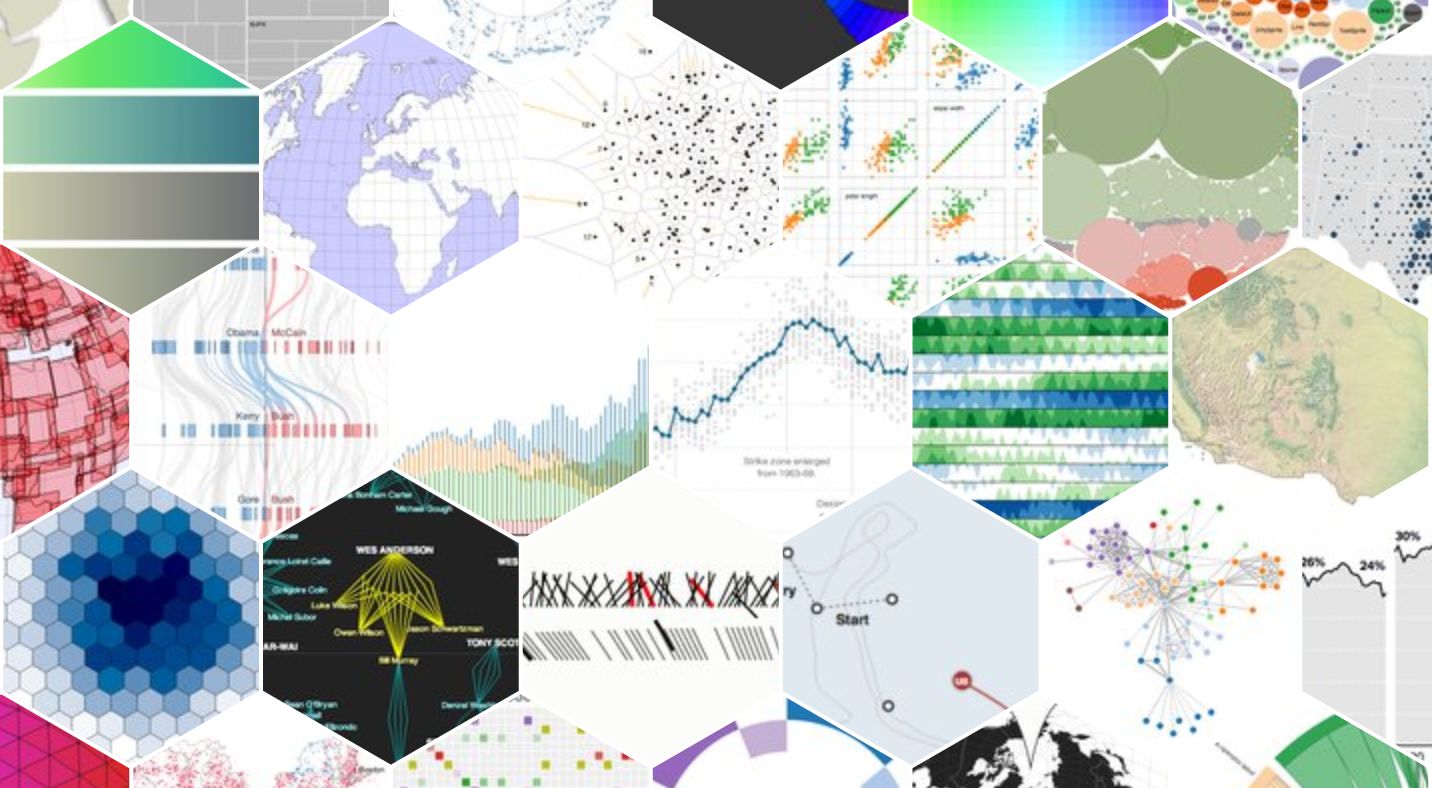
\includegraphics[scale=0.25]{Pictures/Rvisu2}
\end{column}
\end{columns}	
}

% David's Section
%%%%%%%%%%%%%%%%%%%%%%%%%%%%%%%%%%%%%%%%
\section{Basic R Operations}

%\frame[containsverbatim]{
%\frametitle{ImportEIA - Libraries}
%\begin{lstlisting}
%# Load Libraries and Data
%# download data from https://www.eia.gov/electricity/data/eia826/
%library(zoo)
%library(reshape2)
%\end{lstlisting}
%}
\frame[containsverbatim]{
\frametitle{Arithmetic}
\vspace{-0.3cm}\begin{rc}
2 + 3			# add
[1] 5
4 * 5 / 6		# multiply and divide
[1] 3.333333
7^8				# 7 to the 8th power
[1] 5764801
sqrt(2)			# square root
[1] 1.414214
exp(1)			# Euler's constant
[1] 2.718282
pi
[1] 3.141593
5 %/% 2			# 2; integer division
5 %% 2			# 1; modulo division
\end{rc}

}

\frame[containsverbatim]{
	\frametitle{Assignments}
	\vspace{-0.3cm}\begin{rc}
x <- 7*41/pi	# R2L assignment
x				# show entries of x
[1] 91.35494

x = 7*41/pi		# equality assignment (R2L)
x
[1] 91.35494

7*41/pi -> x 	# L2R
x
[1] 91.35494\end{rc}
	
}

\frame[containsverbatim]{
	\frametitle{Object types}
	\vspace{-0.3cm}\begin{rc}
a <- 3; a			# integer
[1] 3

b <- pi; b 			# double
[1] 3.141593

c <- "character"; c	# alternative with '
[1] "character"

d <- (a < 10); d	# logical
[1] TRUE
\end{rc}	
}


\frame[containsverbatim]{
	\frametitle{Logical functions}
\vspace{-0.3cm}\begin{rc}
< 	# smaller
<= 	# smaller or equal
> 	# bigger
>=	# bigger or equal
!= 	# unequal
== 	# logical equal
! 	# logical NOT (unary)
&  	# logical AND (vector)
| 	# logical OR (vector)
&&	# logical AND (no vector)
|| 	# logical  OR (no vector)
\end{rc}	
}

\frame[containsverbatim]{
	\frametitle{Vectors}
	\vspace{-0.3cm}\begin{rc}
a = 1:3
b = 2:4
c(a,b)		# [1] 1 2 3 2 3 4
c(1,1:3)	# [1] 1 1 2 3
array(1,4)	# [1] 1 1 1 1; array(input, dim)  
	\end{rc}	
}

\frame[containsverbatim]{
	\frametitle{More vectors}
	\vspace{-0.3cm}\begin{rc}
seq(1,3)				# [1] 1 2 3
seq(3)					# [1] 1 2 3
seq(1,2,by=0.1)			# [1] 1.1 1.2 1.3 1.4 1.5
seq(1,3,0.5)			# [1] 1.0 1.5 2.0 2.5 3
seq(1,3,length.out = 4)	# [1] 1.00 1.67 2.33 3.00
rep(1:4,2)				# [1] 1 2 3 4 1 2 3 4
rep(1:4,each = 2)		# [1] 1 1 2 2 3 3 4 4 
rep(c(7,9,3), 1:3)		# [1] 7 9 9 3 3 3
	\end{rc}	
}


\frame[containsverbatim]{
	\frametitle{More vectors}
	\vspace{-0.3cm}\begin{rc}
a <- c(2,3,1,4)	# double vector [1] 2 3 1 4
length(a)		# [1] 4
rev(a)			# [1] 4 1
a[<i>]			# returns
a[1:2]			# [1] 2 3
a[-1]			# [1] 3 1 4
a[-c(1,2)]		# [1]
a[a < 3]		# [1] 1 2
which(a == 3)	# [1] 2
a > 1			# [1] TRUE TRUE FALSE TRUE
	\end{rc}	
}


\frame[containsverbatim]{
	\frametitle{More vectors}
	\vspace{-0.3cm}\begin{rc}
a <- letters [1:3]; a
[1] "a" "b" "c"

b <- LETTERS [1:3]; b
[1] "A" "B" "C"

c <- month.abb[1:6]; c
[1] "Jan" "Feb" "Mar" "Apr" "May" "Jun"

d <- month.name[1:12]; d
[1] "January"   "February"  "March"   ...

	\end{rc}	
}

\frame[containsverbatim]{
	\frametitle{More vectors}
	\vspace{-0.3cm}\begin{rc}
a <- c(1,2,3,4) # double vector [1] 1 2 3 4
t(a) # returns d as row vector (transposes d), but is already a matrix
	 [,1] [,2] [,3] [,4]
[1,] 	1 	 2    3	   4
t(t(a)) # column vector, is also matrix 
	  	[ ,1]
	[1,]	1 
	[2,]	2
	[3,]	3
	[4,]	4
	\end{rc}	
}

\frame[containsverbatim]{
	\frametitle{Matrices}
	\vspace{-0.3cm}\begin{rc}
matrix(1:12, nrow=3)
	[,1] [,2] [,3] [,4]
[1,]   1   4    7   10
[2,]   2   5    8   11
[3,]   3   6    9   12
matrix(1:12, nrow=3, ncol=4, byrow = T)
	[,1] [,2] [,3] [,4]
[1,]   1   2    3    4
[2,]   5   6    7    8
[3,]   9  10   11   12
diag(1, nrow=2, ncol=2) # diagonal matrix
     [,1] [,2]
[1,]    1    0
[2,]    0    1
	\end{rc}	
}


\frame[containsverbatim]{
	\frametitle{Merging vectors to matrices}
	\vspace{-0.3cm}\begin{rc}
x = 1:3
y = 4:6
rbind(x,y)
   [,1] [,2] [,3]
x    1    2    3
y    4    5    6
cbind(x,y)
	 x y
[1,] 1 4
[2,] 2 5
[3,] 3 6
	\end{rc}	
}


\frame[containsverbatim]{
	\frametitle{Matrices: Size}
	\vspace{-0.3cm}\begin{rc}
x <- matrix(1:10, 2, 5)
dim(x)			# size of matrix x
col(x)			# column indices of ALL elements
row(x)			# row indices of ALL elements
x[<i>,<j>]		# extract i-th row and j-th column
x[row(x) == col(x)]	# extract the diagonal
	\end{rc}	
}


\frame[containsverbatim]{
	\frametitle{Sums and products}
	\vspace{-0.3cm}\begin{rc}
x = matrix (1:20 ,4 ,5)
sum(x)
[1] 210
prod (x)
[1] 2.432902e+18
colSums(x)
[1] 10 26 42 58 74
rowSums(x)
[1] 45 50 55 60
rowMeans(x)
[1] 9 10 11 12
colMeans(x)
[1] 2.5 6.5 10.5 14.5 18.5
	\end{rc}	
}

\section{Programming}

\frame[containsverbatim]{
	\frametitle{Loops and conditions: FOR}
	\vspace{-0.3cm}\begin{rc}
for (i in 1:4){ print(i) }

for (i in letters[1:4]){ print(i) }

a <- numeric(400) # generate empty a of length 400
for (i in 1:400){ a[i]=i } # fill a with 1:400
# takes much longer than a <- 1:400
	\end{rc}	
}

\frame[containsverbatim]{
	\frametitle{Loops and conditions: WHILE}
	\vspace{-0.3cm}\begin{rc}
i <- 0 
while(i<4){
	i <- i+1
	print(i)
}
	\end{rc}	
}

\frame[containsverbatim]{
	\frametitle{Loops and conditions: REPEAT}
	\vspace{-0.3cm}\begin{rc}
i <- 0;
repeat{
	i <- i+1;
	print(i);
	if (i==4) break
}
	\end{rc}
If no break is given, loops runs forever!
}

\frame[containsverbatim]{
	\frametitle{Loops and conditions: IFELSE}
	
	\texttt{ifelse(boolean check, if-case, else-case)}\\
\begin{rc}
x <- c(6:-4)
sqrt(x) 					# gives warning
sqrt(ifelse(x >= 0, x, NA))	# no warning
	\end{rc}

}


\frame[containsverbatim]{
	\frametitle{Functions}
	
%	\texttt{ifelse(boolean check, if-case, else-case)}\\
\begin{rc}
col.means <- function(input){
	n    = nrow(input)
	ones = 
	return((rep(1,n) %*% input)/n)
}

colMeans(matrix(1:12,3,4))
col.means(matrix(1:12,3,4))
\end{rc}
	
}

\frame[containsverbatim]{
	\frametitle{Task}
	
Write a function that calculates the {\bf column means} of a dataset using the {\bf \texttt{for} loop}.	
}

\section{Data}

\frame[containsverbatim]{
	\frametitle{Load datasets}
	
	\begin{rc}
setwd("C:/...")
setwd("/Users/...")
data <- read.csv("DAX30.csv", sep=",") # data set is a CSV-file
	\end{rc}
}





\end{document}
